%----------------------------------------------------------------------------------------
%	PACKAGES AND OTHER DOCUMENT CONFIGURATIONS
%----------------------------------------------------------------------------------------

\documentclass{article}
\usepackage[english]{babel}
\usepackage[utf8]{inputenc}
\usepackage{fancyhdr} % Required for custom headers
\usepackage{lastpage} % Required to determine the last page for the footer
\usepackage{extramarks} % Required for headers and footers
\usepackage{graphicx} % Required to insert images
\usepackage{lipsum} % Used for inserting dummy 'Lorem ipsum' text into the template
\usepackage{subfigure} % Used for inserting figure side by side
\usepackage{amsfonts,amsmath,amssymb,amsthm}
\usepackage{array, hhline} % Table visual improvements
\usepackage{multirow}
%\usepackage{caption}
%\usepackage{subcaption}
\usepackage{hyperref} % Required to use hyperlinks

% block diagrams
\usepackage{tikz,textcomp}
\usetikzlibrary{shapes,arrows,matrix,fit}
\usetikzlibrary{circuits.ee.IEC}


% Margins
\topmargin=-0.45in
\evensidemargin=0in
\oddsidemargin=0in
\textwidth=6.5in
\textheight=9.0in
\headsep=0.25in 

\linespread{1.2} % Line spacing

\def\code#1{\texttt{#1}}

% Set up the header and footer
\pagestyle{fancy}
\lhead{\hmwkAuthorName} % Top left header
\rhead{\hmwkClass: \hmwkTitle} % Top center header
\chead{} % Top right header
\lfoot{} % Bottom left footer
\cfoot{} % Bottom center footer
\rfoot{Page\ \thepage\ of\ \pageref{LastPage}} % Bottom right footer
\renewcommand\headrulewidth{0.4pt} % Size of the header rule
\renewcommand\footrulewidth{0.4pt} % Size of the footer rule

\setlength\parindent{0pt} % Removes all indentation from paragraphs

%----------------------------------------------------------------------------------------
%	DOCUMENT STRUCTURE COMMANDS
%	Skip this unless you know what you're doing
%----------------------------------------------------------------------------------------

% Header and footer for when a page split occurs within a problem environment
\newcommand{\enterProblemHeader}[1]{
\nobreak\extramarks{#1}{#1 continued on next page\ldots}\nobreak
\nobreak\extramarks{#1 (continued)}{#1 continued on next page\ldots}\nobreak
}

% Header and footer for when a page split occurs between problem environments
\newcommand{\exitProblemHeader}[1]{
\nobreak\extramarks{#1 (continued)}{#1 continued on next page\ldots}\nobreak
\nobreak\extramarks{#1}{}\nobreak
}

\setcounter{secnumdepth}{0} % Removes default section numbers
\newcounter{homeworkProblemCounter} % Creates a counter to keep track of the number of problems

\newcommand{\homeworkProblemName}{}
\newenvironment{homeworkProblem}[1][Problem \arabic{homeworkProblemCounter}]{ % Makes a new environment called homeworkProblem which takes 1 argument (custom name) but the default is "Problem #"
\stepcounter{homeworkProblemCounter} % Increase counter for number of problems
\renewcommand{\homeworkProblemName}{#1} % Assign \homeworkProblemName the name of the problem
\section{\homeworkProblemName} % Make a section in the document with the custom problem count
\enterProblemHeader{\homeworkProblemName} % Header and footer within the environment
}{
\exitProblemHeader{\homeworkProblemName} % Header and footer after the environment
}

\newenvironment{homeworkSection}[1]{ % New environment for sections within homework problems, takes 1 argument - the name of the section
\renewcommand{\homeworkSectionName}{#1} % Assign \homeworkSectionName to the name of the section from the environment argument
\subsection{\homeworkSectionName} % Make a subsection with the custom name of the subsection
\enterProblemHeader{\homeworkProblemName\ [\homeworkSectionName]} % Header and footer within the environment
}{
\enterProblemHeader{\homeworkProblemName} % Header and footer after the environment
}
   
%----------------------------------------------------------------------------------------
%	NAME AND CLASS SECTION
%----------------------------------------------------------------------------------------

\newcommand{\hmwkTitle}{Final Course Project} % Assignment title
\newcommand{\hmwkClass}{Source Coding} % Course/class
\newcommand{\hmwkAuthorName}{Matteo Drago - 1151518} % Your name
\newcommand{\hmwkClassInstructor}{Giancarlo Calvagno} % Teacher/lecturer


%----------------------------------------------------------------------------------------
%	TITLE PAGE
%----------------------------------------------------------------------------------------
\begin{document}
\title{
\vspace{2in}
\textmd{\textbf{\hmwkClass \\ \hmwkTitle}}\\
\vspace{3in}
}
\author{\textbf{\hmwkAuthorName}}
\date{$8^{th}$ June 2018} % Insert date here if you want it to appear below your name

%----------------------------------------------------------------------------------------

\maketitle
\pagenumbering{gobble} % Used to delete the page number on the title page
\pagenumbering{arabic} % Used to reset the page number after the title page
\setcounter{page}{1}

\clearpage 

\section{Abstract}
In this project I built \textbf{coding} and \textbf{decoding} procedures for static color images by means of vector quantization. In order to do this I implemented the quantizer using the \textit{Linde Buzo Gray} algorithm, in the \textit{split} version; the rate \textit{R} will be of 8 bit/pixel for vectors of size \textit{L} = 3, where the three components are the (R,G,B) or the (Y,U,V) representation of the color image at 8x3 bit/pixel.

In the following, after a brief theory overview and the description of the design of the algorithm, I will compare the performance in terms of distortion and PSNR with respect to the results obtained with the JPEG standard.

\section{Data Compression}
The two main components that defines a compression system are:
\begin{itemize}
	\item the \textbf{encoder} which takes as input the message $\mathcal{A}$ (it could be text, image or audio) and produces its coded version, $\mathcal{A}'$;
	\item the \textbf{decoder} which, upon receiving $\mathcal{A}'$, tries to reconstruct the original message $\mathcal{A}$.
\end{itemize}   
The \textit{type} of system changes based on the technique implemented by our encoder/decoder pair; we speak of \textbf{lossless} compression when the decoder is able to perfectly reconstruct the message $\mathcal{A}$ from $\mathcal{A}'$. However, if we want to achieve an higher level of compression we have to trade-off on the quality of the reconstruction at the receiver side and in this case we speak of \textbf{lossy} compression: the receiver is not able to perfectly reconstruct the original message $\mathcal{A}$, but it provides a lower quality version.

While for the lossless compression we evaluate the performances just in terms of \textbf{rate} (i.e. the average number of bits used to represent each sample value), in the lossy scenario we need also to evaluate how much the received message differs from the original one: this metric is called \textbf{distortion}. The relation between these two metrics is described with the \textit{rate-distortion} \cite{rate_dist} theory, a set of rules and guidelines that let us determine, for example, the amount of rate that we can guarantee to the system without exceeding a certain amount of distortion.

Given the two different version of the same message, how can we actually measure the distortion between them? We can use the \textit{squared error} between the input sequence \textit{x} and the reconstructed one \textit{y}, defined as $(x-y)^2$; in alternative we can use the \textit{absolute difference} defined as $|x-y|$. In general, however, average measures are more informative, in fact we define the \textit{mean squared error} as: 
\begin{equation}
\sigma^2_d = \frac{1}{N} \sum_{n = 1}^{N} (x_n - y_n)^2
\end{equation}
which is used also to evaluate another useful metric, the \textit{signal-to-noise ratio}:
\begin{equation}
SNR(dB) = 10log_{10}\frac{\sigma^2_x}{\sigma^2_d}
\end{equation}
where $\sigma^2_x$ is the average squared value of the original message. In the image processing domain there's another important quantity related to the \textit{mse}, which is the \textit{peak-signal-to-noise ratio} defined as: 
\begin{equation}
PSNR(dB) = 10log_{10}\frac{x^2_{peak}}{\sigma^2_d} 
\end{equation}
where $x_{peak}$ is the peak value assumed by the original signal. I'm going to use these measures in order to quantify the quality of the reconstructed image.

Another way for categorizing our compression system is with respect to the type of quantization they implement. If we implement \textbf{scalar} quantization, we have to code one source symbol at a time; using \textbf{vector} quantization instead, we code groups of symbols altogether, with the advantage of obtaining a lower distortion for a given rate (or vice versa, a lower rate for a given limited distortion). As I outlined in the introduction, the aim of this project is the design of a version of the \textbf{LBG} algorithm, which finds a set of representative L-dimensional vectors, that constitute the \textit{codebook} for our vector quantizer. Once the codebook is complete, it is stored both at the encoder and at the decoder side. % in this way, the encoder has just to find the closest code-vector to the pixels and to assign to each pixel the corresponding index of word in the codebook; then, we send through the channel the list of indexes and, once received, the decoder has to do just a table look-up in order to convert the indexes again in the corresponding pixel values.

\section{The Linde-Buzo-Gray algorithm}

Before delving into details, I would like to highlight that the main task of the project is \textbf{codebook} evaluation: all the computational efforts are focused in finding the optimal set of L-vectors that minimize the distortion at the receiver, for a given rate \textbf{R}.

One way of implementing the procedure is to assume the distribution function of the input data $f_X(x)$ as known; so, after a suitable initialization of the codebook, we compute the optimal partition of input samples $ x \in \mathbb{R}^L$. After that we recompute the codebook using our knowledge of $f_X(x)$, we assign to each sample the best codeword and we evaluate the distortion $D^{(n)}$ (\textit{n} indicates the iteration number). We iterate this procedure until the following stopping condition is verified: 
\begin{equation}
\frac{D^{(n-1)} - D^{(n)}}{D^{(n)}} < \epsilon
\end{equation}
where $\epsilon$ is an arbitrary small design parameter. Note that this algorithm guarantees that the distortion \textbf{never increases}, even if it may not be globally minimized.
Given that in this case the probability distribution function is not known a-priori, the initial algorithm needs the following slight change: 

\begin{enumerate}
	\item Start from a codebook of size K. Set $n = 1$ and $ D^{(0)} = \infty $. Assign a suitable value to $\epsilon$; %\textbf{In this case all pixels are represented by this codeword}; 
	\item Partition the dataset with respect to the codebook: to each pixel is assigned the nearest codeword;
	\item Compute the new codewords as centroids of the clusters:
	\begin{equation}
	c_i^{(n)} = \frac{1}{|C_i^{(n)}|} \sum_{x \in C_i^{(n)}} x \quad i = 1,...,K
	\end{equation}
	\item Evaluate the new distortion value:
	\begin{equation}
	D^{(n)} = \frac{1}{|\mathcal{P}|} \sum_{x \in \mathcal{P}} ||x - c_x^{(n)}||_2^2
	\end{equation}
	where $c_x^{(n)}$ is the codeword assigned to the pixel x a the n-th iteration.
	\item If the termination condition described in (4) is met, the computation stops, otherwise increase \textit{n} by one and return to step 2.
\end{enumerate}

We can notice that there are several similarities with the Lloyd's algorithm \cite{Lloyd}, which is also used in pattern recognition when we want to subdivide a dataset of points into \textit{k} representative clusters (in our case the codebook represents the set of centres of different clusters). As for the Lloyd's algorithm, also here the codebook initialization is fundamental in order to guarantee that the algorithm converges to an optimum in considerably less iterations and computational efforts (for Lloyd's initialization, see \textit{kmeans++} \cite{kmeans++}). In past years several techniques were implemented with the aim of optimizing this initial step and in this project I will focus on the \textbf{splitting technique}. Initially we start with a codebook of size 1, where the same codeword is assigned to each pixel. Then, the second codeword is obtained as $ c_2 = c_1 + \delta$ and we apply LBG to the new codebook; when it finishes, we can double the size of the codebook applying $c_{2i} = c_i + \delta$. We iterate this procedure until we reach the desired codebook size (of course we can also obtain sets of odd dimensions, by simply deciding how many additional codewords to create). The reason behind this "iterative doubling" lies on the fact that at each iteration we have the guaranty to start from the optimal version of the codebook, thank to the property of LBG to be optimal.

\section{MATLAB implementation}

%The \textit{end-to-end} environment that I wrote consists of one main script \code{main.m} and three distinct auxiliary functions. 
In this case, the decision of how to pre-process data is fundamental: in my case, I decided to import raw image and work with their RGB representation; in particular I haven't used the \code{uint8} format for the pixels, but I used the \code{im2double} routine instead, in order to avoid mathematical problems. I also stacked all the image pixel rows one on top of the other, in order to use it as a column array (this simplify a lot all operations).

In the design of the procedure described in the previous section there were different issues to be addressed; first of all, the well-known \textbf{empty cell} problem. It may happen that, at some point of LBG, one codeword has no pixels assigned to it: its cluster is empty and it can be seen as an \textit{outlier} of the pixel distribution. In MATLAB I had to avoid this condition because when trying to compute the centroid of each cluster it results in triplets of \code{NaN}.

The routine \code{checkAnyEmptyClt.m} tries to address this problem: it checks if there are any empty sets during a particular iteration. This checking operation, however, takes time if not properly optimized and, after testing different solutions, I decided to use the MATLAB function \code{tabulate}, which takes as input a column array of size \textit{width*length} (parameters of the input image). Each position of the array represents one pixel of the image and each pixel is represented with the index of the respective codeword in the codebook; the output of the function gives complete information on how the array is populated so, after few adjustments, the function returns the index of the \textbf{first} empty cluster on the list. 

Of the course the correspondent codeword must be substituted and, in order to do so, the algorithm uses as candidates the pixels of the \textit{most populated} cluster; the new codeword is picked randomly from this set and as last step all clusters are updated consequently. This step is crucial to understand my implementation of LBG, which can be found in the function \code{LBG.m}: in fact, the algorithm persists on point \textbf{2} described above until all clusters are populated; once all codewords have their assigned pixels, the procedure can continue from point \textbf{3}.

Few details on how I decided to implement the partition strategy: in general, with LBG we assign to a pixel the \textbf{nearest} codeword, which is the one that provides the smaller distortion. Here instead, I decided to write \code{LBG.m} such that a codeword is assigned to a pixel only if: 
\begin{equation}
D_{new} < GD_{old}
\end{equation}
where $D_{new}$ is the distortion between the pixel and the new candidate codeword, $D_{old}$ considers the current assigned codeword and $\mathbf{G}$ is a design parameter to set at the beginning of the simulation. After different tests, I confirmed that this design choice guarantees that the algorithm doesn't get stuck on situations where one pixel keeps on switching from one cluster to another increasing the number of iterations, and so the execution time, without providing any valuable improvement; in fact with this small modification one pixel changes cluster only if using a different codeword introduces a considerable gain. The final choice of \textbf{G} is done considering that also a value too small leads to the problem of coarse approximation (few updates, higher distortion), and in fact we need to find a good trade-off between the number of iterations and the quality of the results (remeber that the standard LBG comes with $G = 1$).
Another possibility, if one wants to avoid the code to be stuck in a loop, is to set a maximum number of iterations after which the routing can proceed with other operations.
I've written also the function \code{distortion.m}, in order to speed up time performances in evaluating the euclidean distance between triplets of pixels.

Once finished with the codebook evaluation we can code the image appropriately: but each pixel is already assigned to a specific cluster (remember the input array that we use in \code{checkAnyEmptyClt.m}), so we just need to rearrange the information that we already have in order to assemble the output image, and to compare the quality of the coded version with the original one.

Just to sum up, the steps are the following:
\begin{itemize}
	\item Image preprocessing and parameters initialization
	\item Codebook evaluation via LBG split
	\item Coding of the image into its quantized version
	\item Study of the differences with the original image
\end{itemize}

\section{Performance Evaluation}
In order to test the algorithm and to evaluate code performances, I used colour images from the dataset in \cite{SIPI}; here all pictures are of size 256x256 or 512x512, while I didn't test higher dimension because the only difference is on the execution time but not on real coding performances. All the images from the dataset are of type TIFF, suitable for our purposes; moreover, after few tests I decided to set $\delta = 0.2$.

\begin{figure}
	\subfigure[Codebook size = 2]
	{
		\includegraphics[scale=.4]{img/1/img_png_1}
	}
	\hfill
	\subfigure[Codebook size = 4]
	{
		\includegraphics[scale=.4]{img/1/img_png_2}
	}
	\hfill
	\subfigure[Codebook size = 8]
	{
		\includegraphics[scale=.4]{img/1/img_png_3}
	}
	\hfill
	\subfigure[Codebook size = 16]
	{
		\includegraphics[scale=.4]{img/1/img_png_4}
	}
	\vfill
		\subfigure[Codebook size = 32]
	{
		\includegraphics[scale=.4]{img/1/img_png_5}
	}
	\hfill
	\subfigure[Codebook size = 64]
	{
		\includegraphics[scale=.4]{img/1/img_png_6}
		\label{fig:complete_1e}
	}
	\hfill
	\subfigure[Codebook size = 128]
	{
		\includegraphics[scale=.4]{img/1/img_png_7}
	}
	\hfill
	\subfigure[Codebook size = 256]
	{
		\includegraphics[scale=.4]{img/1/img_png_8}
		\label{fig:complete_full}
	}
	\caption{256x256 quantized image - $\epsilon = 0.001$, $G = 1$ and $\delta = 0.2$}
	\label{fig:complete_1}
\end{figure}

In order to give a general overview, Figure \ref{fig:complete_1} shows what the quantized image looks like using different codebook sizes, from 2 up to 256. It's clear how the approximation gains in precision as we increase the number of clusters: even if the face and different edges are clearly distinguishable using just 6 bit/pixel, Figure \ref{fig:complete_1e}, the shadows and colour shades of the scarf and flowers are appreciable just with higher rates. 

Before further discussions, it could be useful to spend few lines about what the \textit{rate}, with the intention of keep my considerations consistent. First of all, we should remember that at the beginning our image is a huge matrix of (R,G,B) triplets; each channel can assume values from 0 to 255, and this means that each pixels correspond to 24 bits of information. So, in our scenario the \textit{rate} is the exact amount of bits that we have to use in order to represent one single pixel. The main point of the quantization procedure is that, if we assume the codebook as stored both at the encoder and decoder sides, we just need to send the corresponding index of the codeword in the codebook for each single pixel: in our case, given that the maximum codebook size is 256, we'll send at most 8 bit/pixel, as requested from the problem. 

\begin{figure}
	\centering
	\subfigure[]
	{
		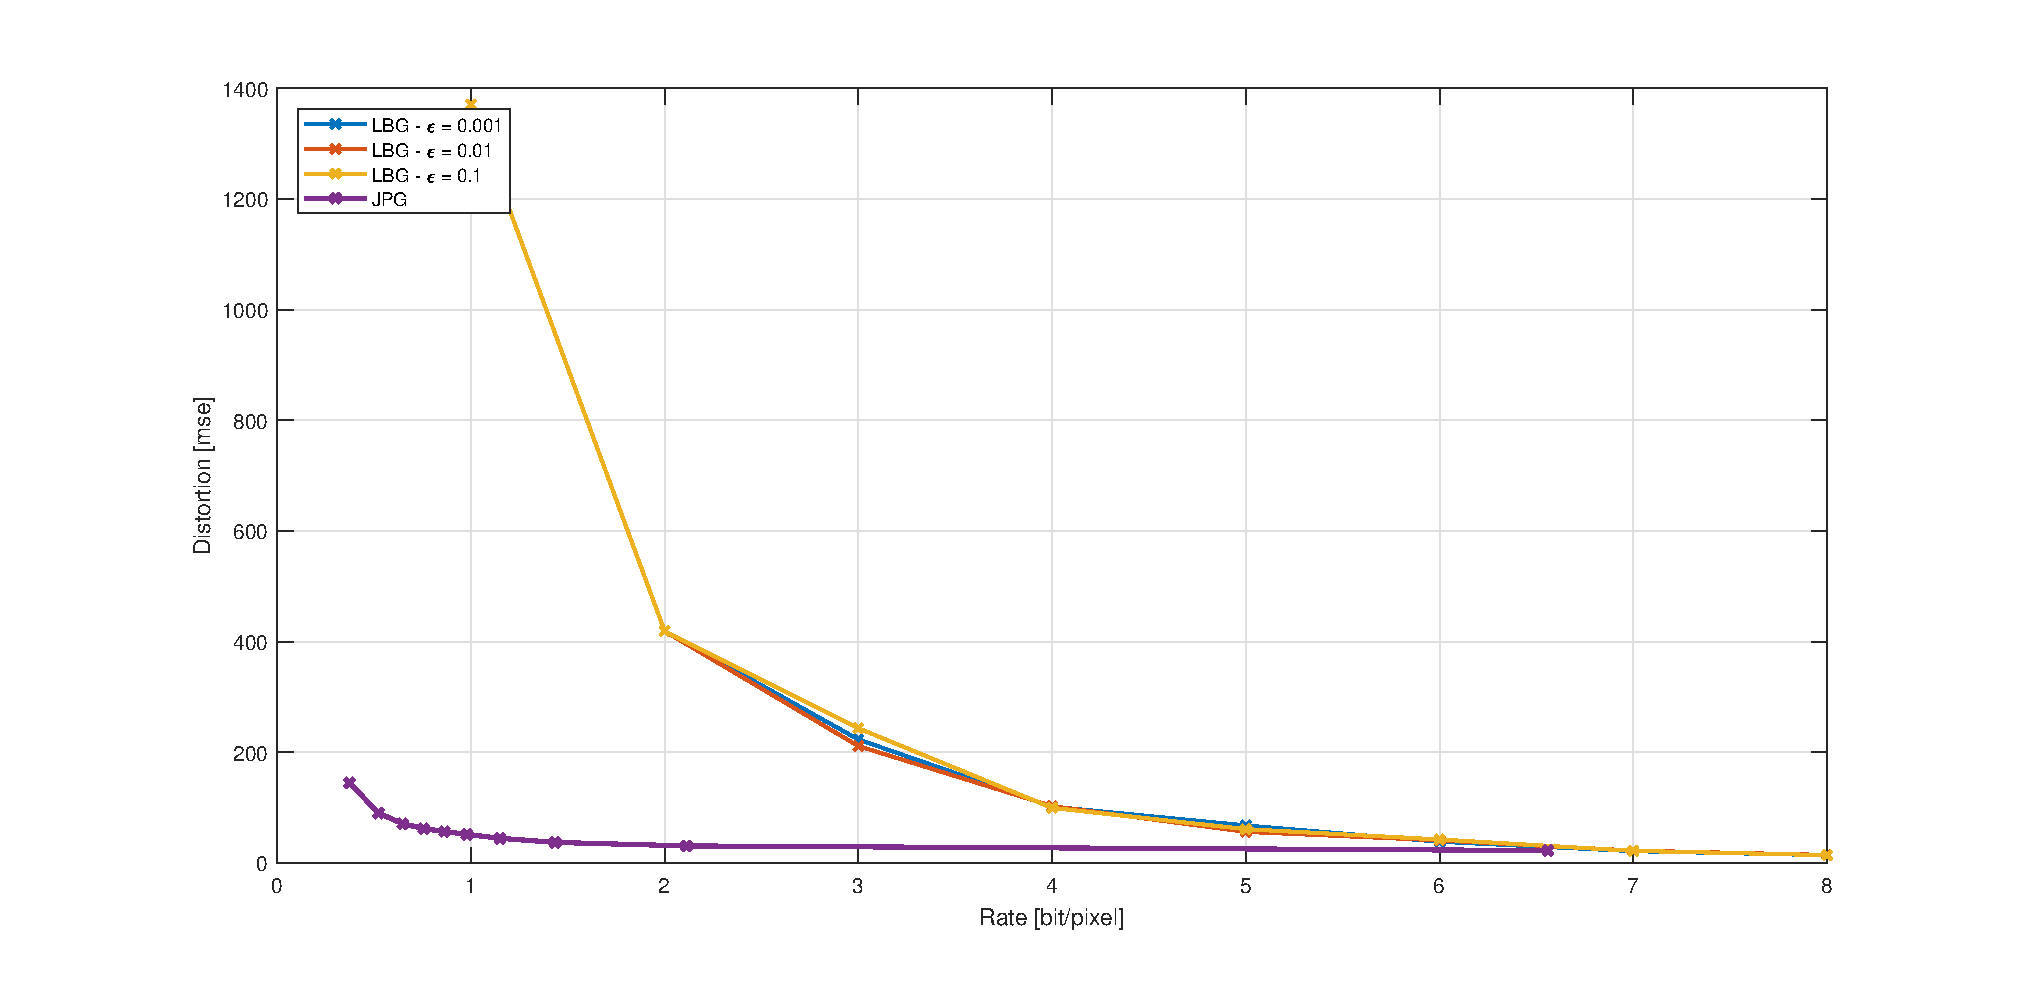
\includegraphics[scale=.4]{img/1/distortion}
		\label{fig:comparison_dist}
	}
	\hfill
	\subfigure[]
	{
		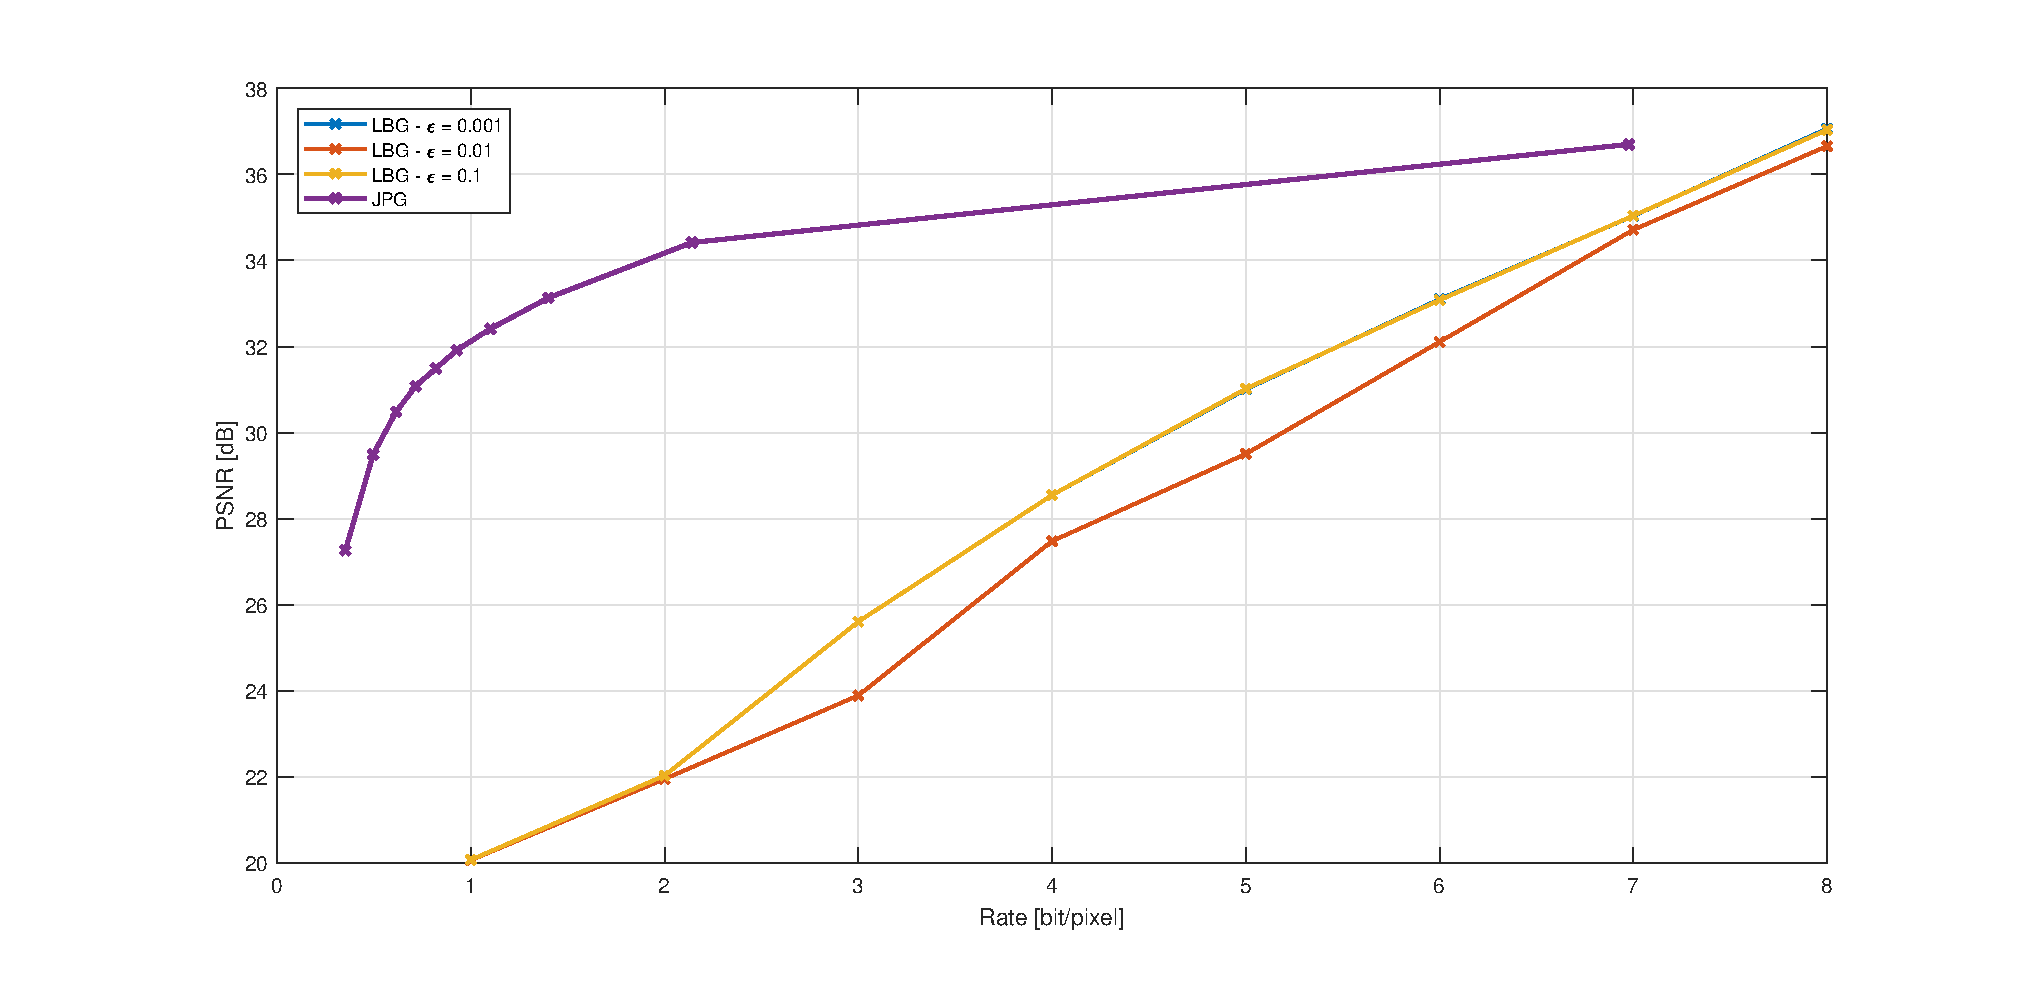
\includegraphics[scale=.4]{img/1/psnr}
		\label{fig:comparison_psnr}
	}
	\caption{Comparison of distortion and PSNR for the image at \ref{fig:complete_full}}
	\label{fig:dist_psnr_1}
\end{figure}
 
With this preamble we can discuss Figure \ref{fig:dist_psnr_1}, where I compared performances in terms of PSNR and distortion (as defined is the second section) in function of the rate and for different values of $\epsilon$. In our scenario we can see how using a lower $\epsilon$ increases performance, in particular at lower rates; changing from $\epsilon = 0.01$ to $0.001$ however doesn't seem to improve, but instead it just increases the price that we have to pay in terms of number of overall iterations as shown in Figure \ref{fig:iterations_1}. The last important point that I want to stress here is about the comparison between this method and the JPEG compression technique. In Figure \ref{fig:dist_psnr_1} we can see as a purple circle what we would have obtained if we would have used JPG: [to be continued]
\begin{figure}
	\centering
	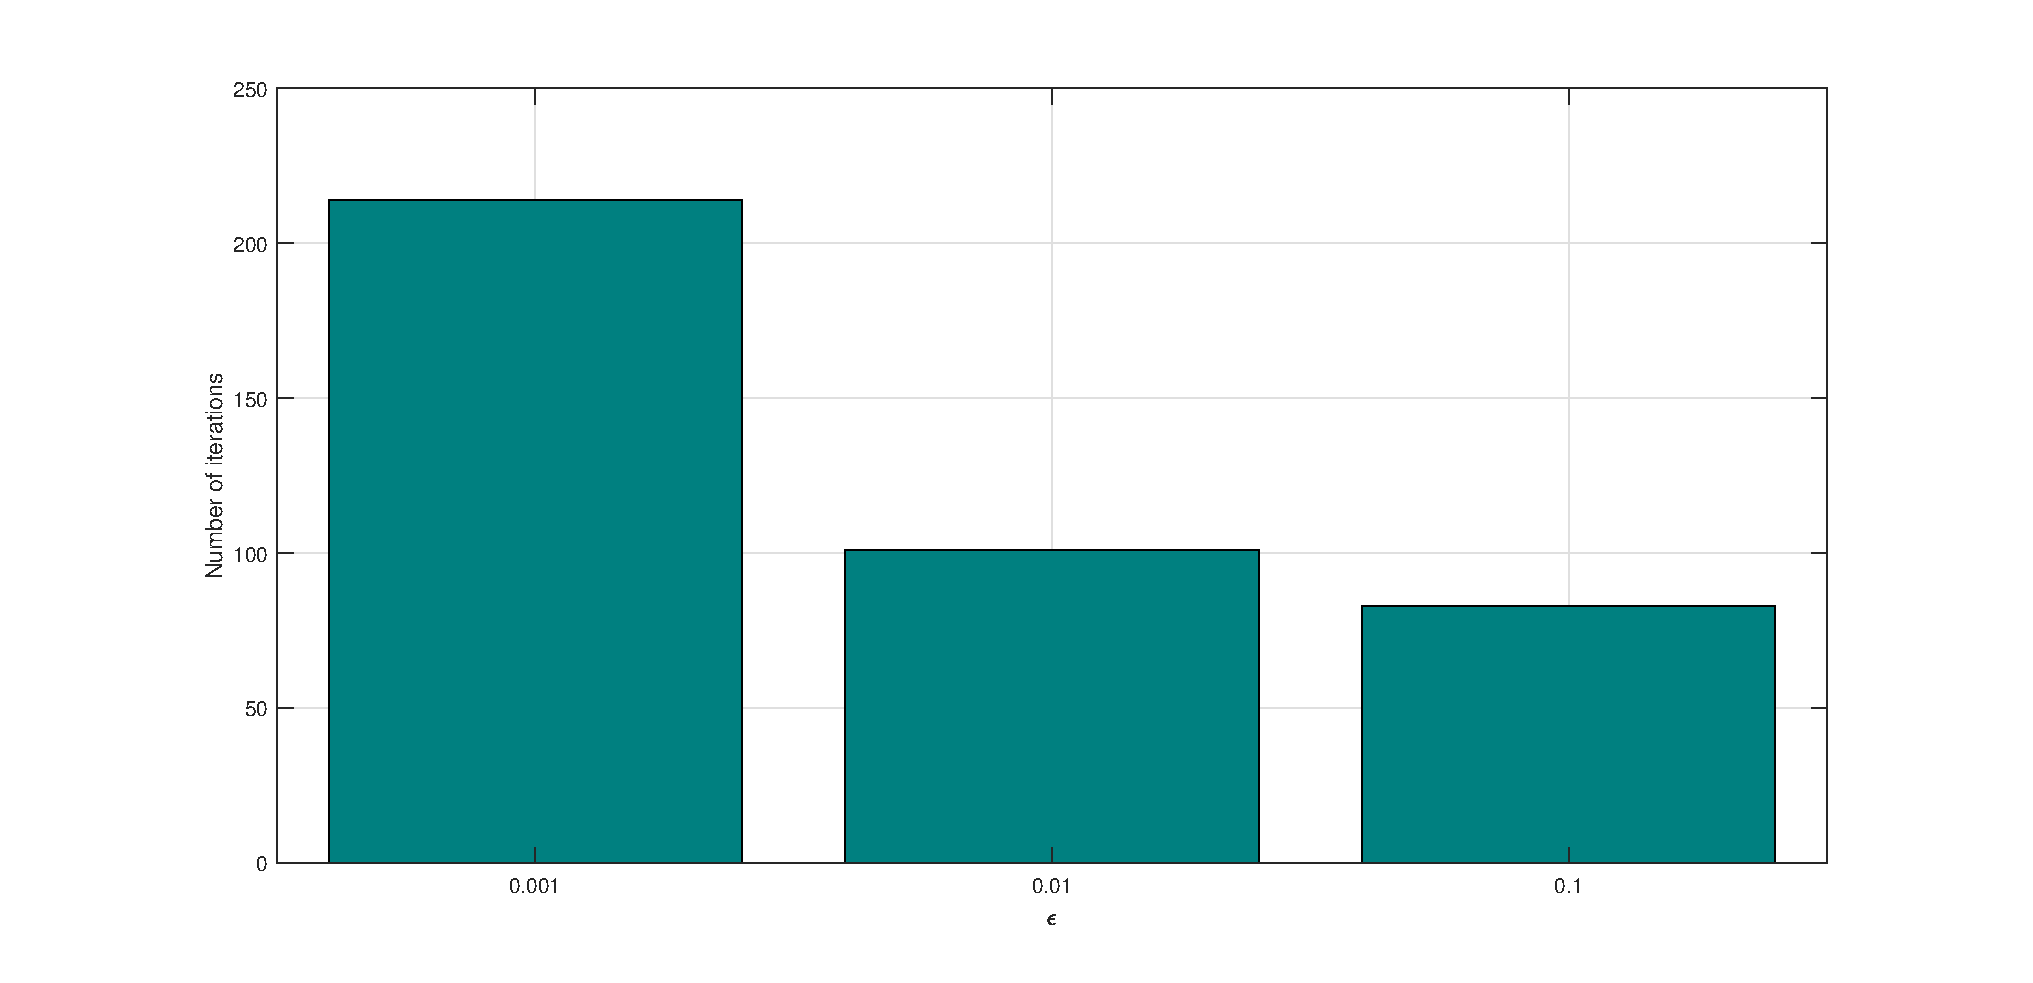
\includegraphics[scale=.4]{img/1/iterations}
	\caption{}
	\label{fig:iterations_1}
\end{figure}


\clearpage

\begin{thebibliography}{9}
		
	\bibitem{rate_dist}
		\textit{Rate Distortion Theory: A Mathematical Basis for Data Compression}
		Tony Berger (1971), Prentice Hall
		
	\bibitem{Lloyd}
		\textit{Least squares quantization in PCM}
		Lloyd, Stuart P. (1982), IEEE Transactions on Information Theory
		
	\bibitem{kmeans++}
		\textit{k-means++: The Advantages of Careful Seeding}
		David Arthur and Sergei Vassilvitskii (2007)
		
	\bibitem{SIPI}
		\textit{SIPI Image Database},
		USC, University of Southern California
	
	\bibitem{TIFF}
		\textit{Tagged Image File Format},
		\href{https://it.wikipedia.org/wiki/Tagged_Image_File_Format}{Wikipedia webpage}
	
	
\end{thebibliography}

\end{document}